\subsection{Vue orthogonale et perspective}
Le moteur graphique permet de changer de mode de vue et permet de passer d'une vue en perspective (active par défaut) à une vue orthogonale.\\
Cette vue est très utilisée notamment dans les logiciels de modélisation 3D faits pour la mécanique.\\
\par
Pour obtenir cette vue, il suffit d'assigner la position de la caméra comme étant la position de l'écran et d'affecter $e_z$ (la direction de la caméra) aux vecteurs directeurs des pixels de l'écran.
\begin{figure}[h]
    \centering
    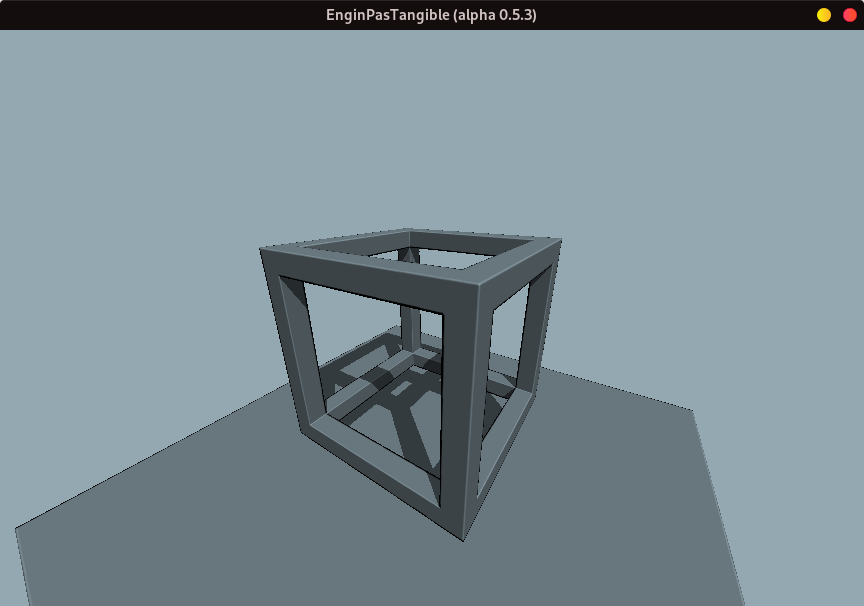
\includegraphics[width=7cm]{images/screens/orthoff.png}
    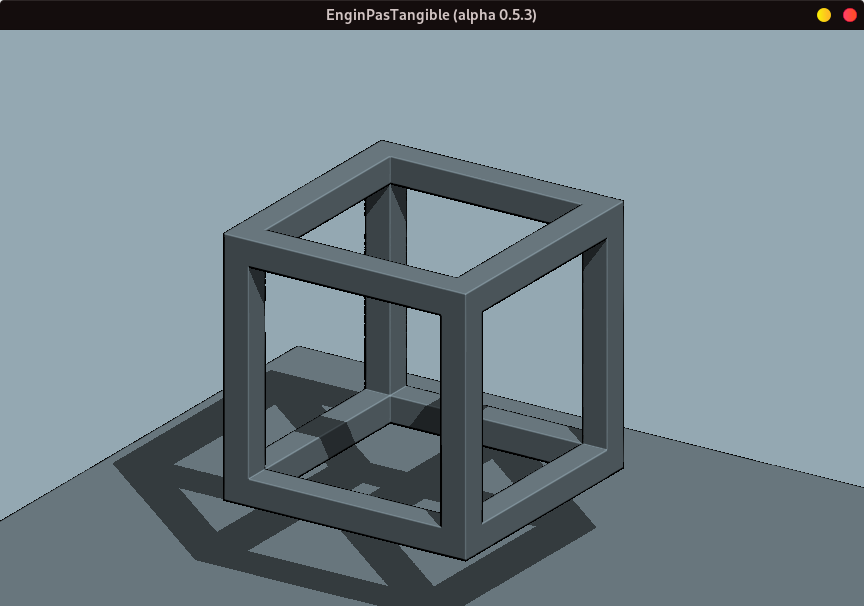
\includegraphics[width=7cm]{images/screens/orthon.png}
    \caption{Différence entre perspective et vue orthogonale}
    \label{fig:orthoview}
\end{figure}